\subsection{Data and Evaluation}
\label{sec:data}
We prepare 3,051 BFCL examples from seven categories at repository revision \texttt{6ea57973c7a6}\footnote{Full revision: \nolinkurl{6ea57973c7a6097fd7c5915698c54c17c5b1b6c8}. The saved setup lists source URLs, hashes, and format changes.}. Each run uses all examples once. Settings were chosen on these examples (no held-out split): $r=3$ on the first run at threshold 0.8, returning the last proposal; then threshold 0.5 (of 0.7 and 0.5) and the first proposal, after \textbf{DMFC} lowered \nolinkurl{gpt-5.4-mini}'s accuracy.

% BEGIN AUTO CATEGORIES
\begin{table}[t]
\centering\footnotesize
\setlength{\tabcolsep}{4pt}
\begin{tabular}{lrrrrr}
\toprule
 & & \multicolumn{2}{c}{\texttt{gpt-5-nano}} & \multicolumn{2}{c}{\nolinkurl{gpt-5.4-mini}}\\
\cmidrule(lr){3-4}\cmidrule(lr){5-6}
Category & Examples & Direct & \textbf{DMFC} & Direct & \textbf{DMFC}\\
\midrule
Simple Python & 400 & 90.8 & 91.3 & 90.5 & \textbf{91.8}\\
Multiple & 200 & 91.0 & 91.5 & 93.3 & \textbf{95.0}\\
Irrelevance & 240 & 27.2 & 78.2 & 87.1 & \textbf{87.9}\\
Live simple & 258 & 74.3 & 77.8 & 77.1 & \textbf{79.8}\\
Live multiple & 1053 & 67.6 & 71.4 & 75.2 & \textbf{77.4}\\
Live irrelevance & 884 & 48.8 & 65.7 & \textbf{80.7} & 79.4\\
Live relevance$^\dagger$ & 16 & 89.6 & \textbf{91.7} & 79.2 & 83.3\\
\midrule
Total & 3051 & 64.1{\scriptsize$\pm$0.3} & 74.8{\scriptsize$\pm$0.3} & 81.1{\scriptsize$\pm$0.2} & \textbf{82.1}{\scriptsize$\pm$0.1}\\
USD/1k & & 0.056 & 0.210 & 0.703 & 1.137\\
\bottomrule
\end{tabular}
\caption{Accuracy (\%) on all BFCL examples, mean of three runs, $r=3$. Bold: highest per row. Total: mean $\pm$ s.d. over runs. USD/1k: cost per 1,000 requests. $^\dagger$Call presence only; not in the total.}
\label{tab:categories}
\end{table}
% END AUTO CATEGORIES

The original Python abstract syntax tree (AST) checker compares function names and arguments with allowed answers, not execution success; irrelevance categories require no call. Live relevance checks only call presence, so the main score, a micro-average, covers 3,035 examples. BFCL's ``multiple'' categories offer several functions but no parallel calls; we exclude parallel, multi-turn, web-search, memory, and execution categories.

\subsection{Models and Methods}
The generator is the Azure OpenAI deployment \texttt{gpt-5-nano} (\nolinkurl{gpt-5-nano-2025-08-07}), with reasoning effort \texttt{none} and at most 4,096 output tokens; \textit{Jev} is pinned to \texttt{jev-1.13.0}. We use Chat Completions through an APIM gateway and System One directly, and convert BFCL schemas to JSON Schema with API-safe function names. Generations cut off at the output limit or blocked by the provider's filter count as wrong. Direct and \textbf{DMFC} also run on the larger, costlier deployment \nolinkurl{gpt-5.4-mini} (snapshot 2026-03-17) with the same settings. Table~\ref{tab:categories} averages three runs per generator, each with new initial proposals.

We compare seven methods, sharing one initial proposal per example. \emph{Direct} uses the initial proposal; \emph{Schema-only} repairs schema errors. \emph{Self-refine} uses generic self-review in all $r$ repairs, not the full Self-Refine method~\cite{madaan2023selfrefine}. \textbf{DMFC-F} and \textbf{DMFC-A} obtain applicable \texttt{Noul} judgments but expose and require only the function or argument verdict, plus schema checks. \textbf{DMFC-A} accepts no call on schema checks alone. \textbf{DMFC-L} shares \textbf{DMFC}'s settings and initial proposal but shows only the latest rejected proposal and feedback. Neither model sees $r$ and nothing runs before the end, so a larger limit only continues trajectories: the first run ran all methods with $r=2$ and continued them to $r=3$; the \textit{Jev} methods ran again at threshold 0.5 (stated in their feedback) from the same initial proposals, \textbf{DMFC} to $r=10$ for Figure~\ref{fig:repairs}. Like \textbf{DMFC}, methods that stop at a passing proposal return the first if none passes.

% BEGIN AUTO RESULTS
\begin{table}[t]
\centering\small
\setlength{\tabcolsep}{2.7pt}
\begin{tabular}{lrrrrr}
\toprule
Method & Call & Func. & Args. & Sec. & USD/1k \\
\midrule
Direct & 63.8 & 74.8 & 81.2 & 1.30 & 0.056 \\
Schema repair & 65.8 & 76.4 & 81.8 & 1.36 & 0.059 \\
Self-refine & 70.0 & 80.3 & 82.2 & 5.47 & 0.265 \\
\textbf{DMFC-F} & 73.2 & 84.5 & 81.4 & 2.24 & 0.172 \\
\textbf{DMFC-A} & 72.5 & 82.6 & \textbf{82.7} & 2.21 & 0.169 \\
\textbf{DMFC-L} & 73.5 & 84.3 & 82.2 & 2.60 & 0.203 \\
\textbf{DMFC} & \textbf{74.6} & \textbf{85.3} & 82.1 & 2.61 & 0.211 \\
\bottomrule
\end{tabular}
\caption{Methods on all BFCL examples (one run, $r=3$, \texttt{gpt-5-nano}). Bold: highest accuracy per column. Call and function accuracy (\%) exclude live relevance; argument accuracy (\%) uses calls with the correct function.}
\label{tab:main}
\end{table}
% END AUTO RESULTS


% BEGIN AUTO REPAIRS
\begin{figure}[t]
\centering
\definecolor{repaircall}{HTML}{2A78D6}
\definecolor{repairfunction}{HTML}{EB6834}
\definecolor{repaircost}{HTML}{52514E}
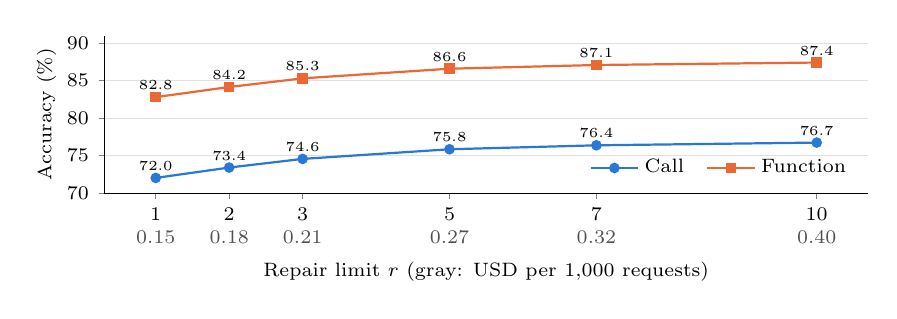
\begin{tikzpicture}
\begin{axis}[scale only axis, width=0.80\columnwidth, height=2.0cm, xmin=0.3, xmax=10.7,
  xtick={1,2,3,5,7,10}, xticklabels={{1\\\color{repaircost}0.15},{2\\\color{repaircost}0.18},{3\\\color{repaircost}0.21},{5\\\color{repaircost}0.27},{7\\\color{repaircost}0.32},{10\\\color{repaircost}0.40}}, xticklabel style={align=center},
  ymin=70, ymax=91, ytick={70,75,80,85,90}, ylabel={Accuracy (\%)}, xlabel={Repair limit $r$ (gray: USD per 1,000 requests)},
  axis x line*=bottom, axis y line*=left, ymajorgrids, grid style={black!12},
  tick label style={font=\scriptsize}, label style={font=\scriptsize}, tick align=outside,
  major tick length=2pt, ylabel style={yshift=-3pt},
  legend style={font=\scriptsize, draw=none, fill=none, at={(0.99,0.03)}, anchor=south east,
  legend columns=2, /tikz/every even column/.append style={column sep=6pt}}]
\addplot[color=repaircall, mark=*, mark size=1.5pt, thick] coordinates {(1,72.0264) (2,73.4102) (3,74.5634) (5,75.8484) (7,76.3756) (10,76.7381)};
\addlegendentry{Call}
\addplot[color=repairfunction, mark=square*, mark size=1.5pt, thick] coordinates {(1,82.8007) (2,84.1516) (3,85.3048) (5,86.5898) (7,87.0840) (10,87.4135)};
\addlegendentry{Function}
\node[font=\tiny, anchor=south, yshift=1.5pt, inner sep=1pt] at (axis cs:1,72.0264) {72.0};
\node[font=\tiny, anchor=south, yshift=1.5pt, inner sep=1pt] at (axis cs:2,73.4102) {73.4};
\node[font=\tiny, anchor=south, yshift=1.5pt, inner sep=1pt] at (axis cs:3,74.5634) {74.6};
\node[font=\tiny, anchor=south, yshift=1.5pt, inner sep=1pt] at (axis cs:5,75.8484) {75.8};
\node[font=\tiny, anchor=south, yshift=1.5pt, inner sep=1pt] at (axis cs:7,76.3756) {76.4};
\node[font=\tiny, anchor=south, yshift=1.5pt, inner sep=1pt] at (axis cs:10,76.7381) {76.7};
\node[font=\tiny, anchor=south, yshift=1.5pt, inner sep=1pt] at (axis cs:1,82.8007) {82.8};
\node[font=\tiny, anchor=south, yshift=1.5pt, inner sep=1pt] at (axis cs:2,84.1516) {84.2};
\node[font=\tiny, anchor=south, yshift=1.5pt, inner sep=1pt] at (axis cs:3,85.3048) {85.3};
\node[font=\tiny, anchor=south, yshift=1.5pt, inner sep=1pt] at (axis cs:5,86.5898) {86.6};
\node[font=\tiny, anchor=south, yshift=1.5pt, inner sep=1pt] at (axis cs:7,87.0840) {87.1};
\node[font=\tiny, anchor=south, yshift=1.5pt, inner sep=1pt] at (axis cs:10,87.4135) {87.4};
\end{axis}
\end{tikzpicture}
\caption{\textbf{DMFC} accuracy (\%) by repair limit $r$: one run continued to $r=10$ and cut at each limit ($r=3$ is Table~\ref{tab:main}).}
\label{fig:repairs}
\end{figure}
% END AUTO REPAIRS

\subsection{Measures, Cost, and Uncertainty}
We report call, function, and argument accuracy (the last given the correct function), fixes and new errors, acceptance, and repairs. We compare repairs with Direct, \textbf{DMFC} with \textbf{DMFC-L}, and the two final-proposal rules on matching examples and initial proposals, bootstrapping example IDs 2,000 times (seed 1729) for 95\% intervals after averaging each example over runs.

Costs count all generation and verification work, including the growing history and the shared initial call; times are mean API seconds without retry waits. Prices in USD per million uncached/\allowbreak cached/\allowbreak output tokens are 0.05/\allowbreak 0.005/\allowbreak 0.40 for \texttt{gpt-5-nano} and 0.75/\allowbreak 0.075/\allowbreak 4.50 for \nolinkurl{gpt-5.4-mini}; \textit{Jev} input costs \$0.042 (output free), without gateway fees; one filtered generation without usage is left out.

\subsection{Results}
In Table~\ref{tab:categories}, \textbf{DMFC} raises mean accuracy from 64.1\% to 74.8\% (paired difference 10.7 points, 95\% interval 9.7--11.6; per run 10.8, 10.7, 10.4). Per run, it fixes 323--337 wrong initial proposals, breaks 7--10, and averages 0.64--0.65 repairs; 84--85\% of examples pass, 84--85\% of them correctly. Other numbers are from the first run unless stated.

% BEGIN AUTO RULES
\begin{table}[t]
\centering\footnotesize
\setlength{\tabcolsep}{4pt}
\begin{tabular}{lrrrr}
\toprule
Generator & Direct & Last & First & First $-$ last\\
\midrule
\texttt{gpt-5-nano} & 64.1 & \textbf{75.1} & 74.8 & $-$0.35 [$-$0.68, $-$0.03]\\
\nolinkurl{gpt-5.4-mini} & 81.1 & 80.7 & \textbf{82.1} & +1.37 [0.93, 1.82]\\
\bottomrule
\end{tabular}
\caption{Call accuracy (\%), mean of three runs, when \textbf{DMFC} returns the last or the first proposal if none passes. First $-$ last: paired difference [95\% interval].}
\label{tab:rules}
\end{table}
% END AUTO RULES

\paragraph{Returning the first proposal.}
The rules differ only when no proposal passes; returning the last then makes unverified changes, which per run fix 26--33 calls and break 16--22 with \texttt{gpt-5-nano} but fix 10--14 and break 53--55, mostly correct no-calls, with \nolinkurl{gpt-5.4-mini}. Keeping only accepted changes gains 1.4 points for \nolinkurl{gpt-5.4-mini} and costs \texttt{gpt-5-nano} 0.4 (Table~\ref{tab:rules}).

\paragraph{A larger generator.}
Without \textit{Jev}, \nolinkurl{gpt-5.4-mini} reaches 81.1\%, 6.4 points above \textbf{DMFC} with \texttt{gpt-5-nano} (95\% interval 5.1--7.7), at 3.3 times the cost and under half the time. \textbf{DMFC} raises it in every run, by 1.0 point on average (95\% interval 0.5--1.5); per run, it fixes 55--66 calls and breaks 27--39, mostly no-calls turned into accepted calls.

\paragraph{Comparison of methods.}
In Table~\ref{tab:main}, every repair method beats Direct (paired 95\% intervals above zero): schema repair by 2.0 points, self-refine 6.3, \textbf{DMFC-F} 9.5, \textbf{DMFC-A} 8.7, and \textbf{DMFC-L} 9.8. Self-refine makes four proposals per request yet trails the \textit{Jev}-based methods (1.4 to 1.6).

\paragraph{Why no-call cases gain most.}
Direct calls the one, unrelated function in 179 of 240 Irrelevance examples. \textit{Jev} separates these from the 61 correct no-calls (median function probability 0.09 vs.\ 0.95), and the generator withholds 126 of 156 rejected calls; in live irrelevance, separation is weaker (0.53 vs.\ 0.87), and 160 of 379 are withheld. Where reference calls exist, \textbf{DMFC} rejects 216 of 463 wrong initial calls but fixes only 51: a verdict flags a wrong call, not the right one.

\paragraph{More repairs.}
In Figure~\ref{fig:repairs}, $r=10$ reaches 76.7\%, at 1.6 times the time and 1.9 times the cost of $r=3$; later passing proposals fix 70 examples (59 by withholding a call) and break 4.

\paragraph{Records as in-context examples.}
Each record pairs a call with \textit{Jev}'s verdict, so the history acts as labeled in-context examples, made without reference answers in 0.19~s per label at about \$0.06 per 1,000. As in many-shot learning~\cite{agarwal2024manyshot}, more examples help: with the same attempts, the full history beats the latest record by 1.1 points (\textbf{DMFC} minus \textbf{DMFC-L}, 95\% interval 0.4--1.7), though all are failed attempts at one request.

\subsection{Study Limits}
The verifier can accept a wrong call or share the generator's mistake, and feedback can introduce or reinforce errors. We use two generators, one verifier, and mostly English single-turn requests; Table~\ref{tab:main} and Figure~\ref{fig:repairs} come from one run, and public examples may appear in training data. Ten documented annotation errors stay. Settings were chosen on these examples, so gains may be optimistic; effort \texttt{none} is untuned, and one common limit may favor some methods.
